\chapter{Fejlesztői dokumentáció} % Developer guide
\label{ch:impl}

Ez a fejezet fejlesztőknek nyújt segítséget a ScrumHelper feltérképezésében. Az alfejezetek kifejtik az alkalmazás felépítését, részletesen leírják a különböző rétegeinek (Adatbázis-Szerver-Nézet) osztályait és függvényeit. A vizuális segítséghez különböző diagrammokat is tartalmaz (osztály-, csomag-, felhasználói esetek diagram). A fejezet végén egy tesztforgatókönyv ad részletes leírást a teszt esetek és azok eredményeiről.

\section{Konfiguráció, fejelsztői környezet}
\label{config}

A futtatáshoz szükséges előkövetelmények a felhasználói dokumentáció \ref{install}. alfejezetében olvashatók. A dolgozatt keretein belül csak a lokális szerveren való konfigurálás és futtatás lesz részletezve. A különböző szervergépeken való futtatáshoz részletesebb információt a hivatalos Django dokumentációban lehet találni. Utóbbi eset külön konfigurációt igényel a wsgi.py, illetve asgi.py file-ok és környezeti változók megfelelő beállításának segítségével \footnote{wsgi szerver: \url{https://docs.djangoproject.com/en/3.0/howto/deployment/wsgi/} asgi szerver: \url{https://docs.djangoproject.com/en/3.0/howto/deployment/asgi/}}.  

Ahhoz, hogy lokálisan futtatni tudjuk a szervert, először is a ScrumHelper/ScrumHelper/setting.py file-ban kell beállítanunk a DATABSES változót. A pontos beállításai eltérőek a különböző adatbázisok esetében, ehhez részletes segítséget nyújt a hivatalos Django dokumentáció. Alább  egy PostgreSQL adatbázis konfigurációja látható:

\lstset{caption={Konfiguráció PostgreSQL adatbázis használatához}, label=src:settingsconf}
\begin{lstlisting}[language={python}]

DATABASES = {
    'default': {
        'ENGINE': 'django.db.backends.postgresql',
        'NAME': 'database name',
        'USER': 'database user',
        'PASSWORD': 'password',
        'HOST': '127.0.0.1',
        'PORT': '5432',
    }
}

\end{lstlisting}

Ha ez megfelelően van beállítva, akkor a ScrumHelper fő mappába navigálva kell lefuttatni a" python manage.py migrate" parancsot minden első futtatásnál a szükséges adatbázis struktúra kialakításához(illetve ha fejlesztés során olyasmi változik, amely érinti az adatbázis struktúrát, akkor a makemigrations-t is le kell a migrate parancs előtt futtatni). Ezután a "python manage.py runserver" elindítja a lokális szervert a localhost:8000-es portján. Superuser-t, azaz minden jogosultsággal rendelkező felhasználót a szerver futtatása nélkül lehet generálni: "python manage.py createsuperuser" paranccsal, megadva a felhasználónevet és jelszavat utána.

A TIMEZONE változóban adható meg az időzóna. Az egyes projektekhez feltöltött fájlokat a MEDIA\_ROOT konfigurációs változóbeli elérési úton elhelyezkedő mappába menti (ez alapból a ScrumHelper/media könyvtárra mutat). Ugyanezen az elven kezeli a statikus fájlokat is a keretrendszer, ennek a környezeti változója a STATIC\_ROOT.

Fontos, hogy mielőtt az alkalmazás valós, produkciós használatba kerülne szükséges a DEBUG változót False, azaz hamisra állítani (biztonásgi okokból).

A Django nem rendelkezik saját fejlesztői környezettel, így bármely Pythonhoz fejlesztésre alkalmas IDE használható. Például a Visual Studio Code rendelkezik minden bővítménnyel, amely szükséges lehet egy Django alkalmazás futtatásához és egyéb "kényelmet" segítő funkciókkal is (szintaxis ellenőrzés/kiemelés Pythonhoz/HTML-hez/CSS-hez/JavaScript-hez és a Django templétekhez). A szükséges szoftverek (\ref{install}) megléte mellett akár egy egyszerű szövegszerkeztő alkalmazás is elegendő (de célszerűbb valameilyen integrált fejlesztői környezetet használni).

\section{Funkcionális terv}

Az \ref{fig:usecase}. ábrán egy felhasználói eset diagram mutatja be az alkalmazás funkcióit:

\begin{figure}[H]
	\centering
	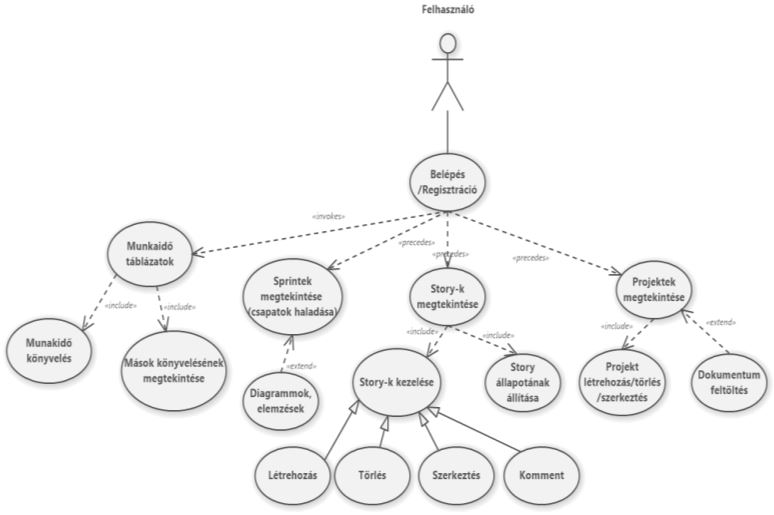
\includegraphics[width=1\textwidth,height=300px]{usecase}
	\caption{Felhasználói eset diagram}
	\label{fig:usecase}
\end{figure}

\section{Struktúrális felépítés}

A ScrumHelper egy MVC (Model-View-Controller) alkalmazás, bár a hivatalos Django dokumentációban az MTV (Model-Template-View) kifejezést használják, mivel ezt gondolják pontosabb leírásának. Tekintve, hogy Djangoban írodott az alkalamzás, ezért ebben a dokumentációban is utóbbi analógia a mérvadó. Ez azt jelenti, hogy három rétegből tevődik össze: egy Model rétegből, amely az adatbázist hivatott reprezentálni, egy View rétegből, amely az adatot reprezentálja (ez alatt azt értjük, amit az adatbázisből kigyűjtött, nem feltétlenül a felhasználó számára megjelnített adatot), valamint a különböző template-ek renderelését is végzi, továbbá egy Template rétegből, mely leírja, hogyan legyen az adat megjelenítve a felhasználó számára.

\begin{figure}[H]
	\centering
	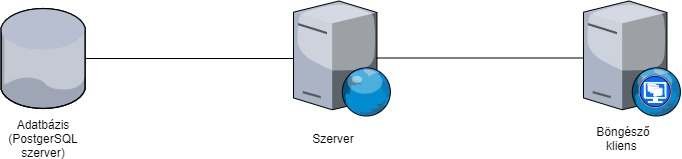
\includegraphics[width=1\textwidth,height=125px]{architecture}
	\caption{Az alkalamzás rétegei: egy adatbázis, egy szerver, ami kinyeri belőle az adatot és továbbítja a nézetnek, valamint a nézet amit a böngészőben láthatunk.}
	\label{fig:architecture}
\end{figure}

A django alkalmazások úgynevezett applikációkból állnak, amelyek a moduláris felépítést segítik elő. Ezek gyakorlatilag a python nyelvből ismert csomagokkal -package-ekkel- egyeznek meg. A \ref{fig:packages}. ábra szemléletesebben bemutatja ezen applikációkat (modulokat) és azok kapcsolatait:

\begin{figure}[H]
	\centering
	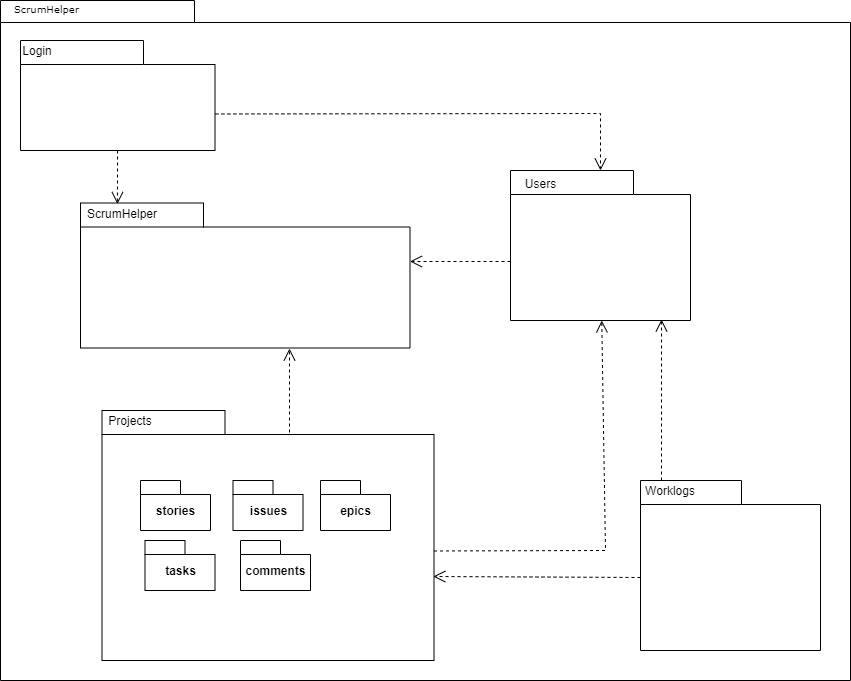
\includegraphics[width=1\textwidth,height=300px]{scrumhelperPackage}
	\caption{Csomagdiagramm}
	\label{fig:packages}
\end{figure}

\pagebreak

\begin{itemize}
 	\item Ahogy az ábrán is látható, a fő csomag a ScrumHelper. Ez fogja össze működésben az alkalamzást.
	\item A legnagyobb applikáció a "Projects", ugyanis ez tartalmazza egyben a "Stories", "Tasks", "Issues", "Comments", "Epics" applikációkat is.
	\item A felhasználók kezelésével foglalkozó csomag a "Users" és részben a "Login". Utóbbi a ki- és bejelentkeztetésre, valamint a felhasználók regisztrálására és szerkeztésére szolgál.
	\item Egy kisebb alkalmazás, a "Worklogs" adja a modell szintű reprezentációját a munkaidő naplónak.
\end{itemize}

Ezek implementáció, részletei a későbbi alfejezetekben olvashatóak. 

\section{Adatbázis réteg}
\label{dbmodels}

A django keretrendszernek köszönhetően az alapkonfigurációt leszámítva nem számít, hogy milyen adatbázissal dolgozunk. A ScrumHelper fejelsztése során a nyílt-forráskódú PostgreSQL-re esett a választás, de a python modellek és az adatbázis lekérdezések függetlenek attól, hogy milyen adatbázist használunk. Ha csak egy kis, egyszerű alkalmazás megvalósítása a cél akkor érdemesebb például SQLite adatbázist használni, tekintve, hogy az csak egy lokális fájlban tárolja az adatokat, könnyebb menedzselni. A PostgreSQL (a MySQL, Oracle, MariaDB mellett) jobb döntésnek bizonyul nagyobb méretű alkalmazások esetén. 

Az egyes adatbázis táblákat (entitásokat) egy-egy modell reprezentál a forráskódban. Ezek a django.db.models.Model osztályból vannak származtatva. Az egyes modellek attribútumai egy-egy oszlopot reprezentálnak a táblában. A django dokumentációban\footnote{django modell típusosztályok: \url{https://docs.djangoproject.com/en/3.0/ref/models/fields/}} részletes leírás található arról, mely mezőtípusokhoz milyen paramétereket lehet megadni ahhoz, hogy minél jobban testreszabhassuk a mező tulajdonságait. Van lehetőség modell szintű metódusokat is definiálni ugyanúgy, mint a python osztályoknál (hiszen ezek is python osztályok), de ezek nem lesznek jelen az adatbázisban. A modell szinten jellemzően csak egyszerűbb metódusokat szokás definiálni, mint például az \textit{\_\_str\_\_()} felüldefiniálása a felsőbb rétegek segítségéül, vagy az \textit{\_\_init\_\_} inicializációs függényt. Érdemes azonban kerülni az ilyen megoldásokat, hogy minél jobban elszeparálhatóak legyenek az egyes rétegek.  A következő alfejezetekben részletes információk találhatóak az egyes modellekről.

\subsection{Felhasználó kezelés: Users, Login modellek}

\begin{figure}[H]
	\centering
	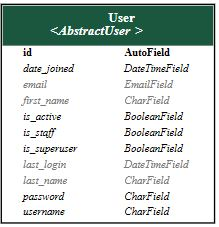
\includegraphics[scale=1.5]{userModel}
	\caption{User modell diagrammja}
	\label{fig:usermodel}
\end{figure}

A \textbf{django.contrib.auth.models.User} modell reprezentál egy-egy felhasználót. Ez magában a keretrendszerben megtalálható. Elég sokoldalú, de van lehetőség kiegészíteni, esetlegesen helyettesíteni saját megvalósítással is. Kiegészítésre példa a \textbf{Profile} modell osztály a users applikációban. Egy \textbf{OneToOneField} segítségével és szignálokkal (\textit{create\_user\_profile} és \textit{save\_user\_profile}) tudjuk az eredeti \textbf{Users} osztályhoz kötni. A szignálok azért szükségesek, mert így tud a modell reagálni az eredeti modell esetleges változásaira (létrehozás, módosítás, törlés). A mezők:

\begin{itemize}
	\item \textit{id}: mezőazonosító (alapvetően generált)
	\item \textit{date\_joined}: beregisztrálás dátuma
	\item \textit{email}: email cím
	\item \textit{first\_name}: keresztnév
	\item \textit{is\_active}: nem zárolt-e a felhasználó (azaz inaktív)
	\item \textit{is\_staff}: adminisztrátor-e
	\item \textit{is\_superuser}: Minden jogosultsággal rendelkező felhasználó-e
	\item \textit{last\_login}: utolsó bejelentkezés dátuma
	\item \textit{last\_name}: vezeték név
	\item \textit{password}: jelszó (hashelve, azaz kódolva)
	\item \textit{username}: felhasználónév
\end{itemize}

A \textbf{Login} modul nem rendelkezik külön adatbázis reprezentációval, mivel a \textbf{User} modelljét használja föl.

\subsection{Projekt modell}

\begin{figure}[H]
	\centering
	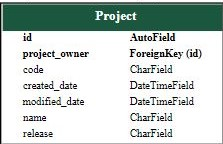
\includegraphics[scale=1.5]{projectModel}
	\caption{Project modell diagrammja}
	\label{fig:projectmodel}
\end{figure}

A \textbf{Projects} applikáció saját adatbázis modellje a \textbf{Project}:

\begin{itemize}
	\item \textit{id}: mezőazonosító (alapvetően generált)
	\item \textit{project\_owner}: a projektet létrehozó felhasználó (idegen kulcs a \textbf{Users} táblára)
	\item \textit{code}: a projekt 6 karakter hosszú kódja (egyedi kell legyen)
	\item \textit{created\_date}: a létrehozás dátuma
	\item \textit{modified\_date}: az utolsó módosítás dátuma
	\item \textit{name}: a projekt neve (maximum 50 karakter hosszú)
	\item \textit{release}: a Release neve (maximum 10 karakter hosszú)
\end{itemize}

Rendelekezik egy \textit{documents} attribútummal is, mely egy \textbf{ManyToManyField} típusú mező, azaz több idegen kulcs kapcsolatot fog egybe (erre a célra a django automatikusan létrehoz egy táblát, amelyben benne lesznek ezek az összekapcsolások) a \textbf{Documents} modell táblájának \textit{id} mezőjével. Ennek seígtségével kapcsolódik egy adott projekthez több dokumentum is.

\begin{figure}[H]
	\centering
	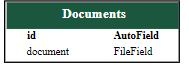
\includegraphics[scale=1.5]{documentModel}
	\caption{Documents modell diagrammja}
	\label{fig:docmodel}
\end{figure}

A \textbf{Documents} modell rendelkezik egy \textit{document} attribútummal, mely \textbf{FileField} típusú. Ez a típusosztály reprezentálja Djangoban a fájl mezőket az adatbázisban. A fájl relatív elérési útját menti le az adatbázisba. Jelen alkalmazásban a \textit{documents/} mappát használja, de ez is konfigurálható a \textit{projects.models.project\_directory\_path(instance, filename)} függvény segítségével. A visszatérési értékben (amely egy string) lehet megadni az elérési utat.

\subsection{Epic modell}

\begin{figure}[H]
	\centering
	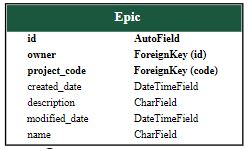
\includegraphics[scale=1.5]{epicModel}
	\caption{Epic modell diagrammja}
	\label{fig:epicmodel}
\end{figure}

Az \textbf{Epic} a \textit{project\_code} mezővel kapcsolódik a \textbf{Project} tábla \textit{code} mezőjéhez. Egy projekthez több több epic is tartozhat, de egy epic csak egy projekthez kapcsolódhat. Ha a projekt törlődik, vagy a létrehozó felhasználó, akkor az összes epic is amelyek hozzá tartoznak. A modell mezői:

\begin{itemize}
	\item \textit{id}: mezőazonosító (alapvetően generált)
	\item \textit{owner}: az epic-et létrehozó felhasználó (idegen kulcs a \textbf{Profile} táblára)
	\item \textit{project\_code}: a projekt 6 karakter hosszú kódja (idegen kulcs, a \textbf{Project} tábla \textit{code} mezőjére mutat)
	\item \textit{created\_date}: a létrehozás dátuma
	\item \textit{modified\_date}: az utolsó módosítás dátuma
	\item \textit{name}: az epic neve (maximum 50 karakter hosszú)
	\item \textit{description}: egy leírás az epic-ről (maximum 250 karakter hosszú)
\end{itemize}

\subsection{Story modellje}

\begin{figure}[H]
	\centering
	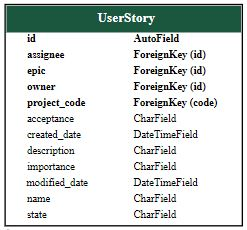
\includegraphics[scale=1.5]{storyModel}
	\caption{Story modell diagrammja}
	\label{fig:storymodel}
\end{figure}

A \textbf{UserStory} több táblához is rendelkezik idegen kulccsal: kapcsolódik egyrészt a projekthez, amely alatt létrehozták, kapcsolódik továbbá a felhasználóhoz, aki létrehozta, illetve akihez rednelve van (utóbbi opcionális), valamint kapcsolódik egy epic-hez (ez is opcionális). Egy story csak addig létezik, amíg a projekt is, amely alatt létehozták, avagy ki nem törlik. Ha epic-hez van rendelve és töröljük, akkor csak kinullázódik azon mezője. Abban az esetben, ha a felhasználót töröljük, aki létrehozta a story-t, akkor is törlődik. A modell mezői:

\begin{itemize}
	\item \textit{id}: mezőazonosító (alapvetően generált)
	\item \textit{assignee}: idegen kulcs a hozzárendelt felhasználóra (lehet üres, \textbf{User} tábla)
	\item \textit{epic}: idegen kulcs az \textbf{Epic} táblára (lehet üres)
	\item \textit{owner}: az story-t létrehozó felhasználó (idegen kulcs a \textbf{Profile} táblára)
	\item \textit{project\_code}: a projekt 6 karakter hosszú kódja (idegen kulcs, a \textbf{Project} tábla \textit{code} mezőjére mutat)
	\item \textit{acceptance}: feltételek leírása, amelyeknek teljesülnie kell (például teszt során, maximum 50 karakter)
	\item \textit{created\_date}: a létrehozás dátuma
	\item \textit{modified\_date}: az utolsó módosítás dátuma
	\item \textit{name}: a story neve (maximum 50 karakter hosszú)
	\item \textit{description}: egy leírás a story-ról (maximum 250 karakter hosszú)
	\item \textit{importance}: fontosság (Low, Medium, High)
	\item \textit{state}: aktuális állapot (OPEN, IN PROGRESS, TESTING, DONE, CLOSED)
\end{itemize}

Rendelkezik egy \textit{comment} mezővel is, amely több kommentet is össze kapcsol egy \textbf{UserStory}-val (\textbf{ManyToMany} reláció, külön kapcsolati táblával). Ugyanilyen kapcsolatban áll a \textbf{Worklog} táblával is a \textit{work\_log} mezőn keresztül.

\subsection{Task modellje}

\begin{figure}[H]
	\centering
	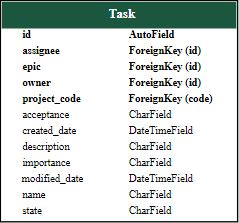
\includegraphics[scale=1.5]{taskModel}
	\caption{Task modell diagrammja}
	\label{fig:taskmodel}
\end{figure}

A \textbf{Task} modell felépítése szinte megegyezik a \textbf{UserStory}-éval. Ugyanúgy egy projekthez, esetlegesen egy epic-hez és a felhasználó(k)hoz kapcsolódik. Az eltérés a státuszaiban van: csak OPEN (nyitott), DONE(kész) és CLOSED(lezárt) lehet. A mezői:

\begin{itemize}
	\item \textit{id}: mezőazonosító (alapvetően generált)
	\item \textit{assignee}: idegen kulcs a hozzárendelt felhasználóra (lehet üres, \textbf{User} tábla)
	\item \textit{epic}: idegen kulcs az \textbf{Epic} táblára (lehet üres)
	\item \textit{owner}: az task-ot létrehozó felhasználó (idegen kulcs a \textbf{Profile} táblára)
	\item \textit{project\_code}: a projekt 6 karakter hosszú kódja (idegen kulcs, a \textbf{Project} tábla \textit{code} mezőjére mutat)
	\item \textit{acceptance}: feltételek leírása, amelyeknek teljesülnie kell (például teszt során, maximum 50 karakter)
	\item \textit{created\_date}: a létrehozás dátuma
	\item \textit{modified\_date}: az utolsó módosítás dátuma
	\item \textit{name}: a task neve (maximum 50 karakter hosszú)
	\item \textit{description}: egy leírás a task-ról (maximum 250 karakter hosszú)
	\item \textit{importance}: fontosság (Low, Medium, High)
	\item \textit{state}: aktuális állapot (OPEN, DONE, CLOSED)
\end{itemize}

Rendelkezik egy \textit{comment} mezővel is, amely több kommentet is össze kapcsol egy \textbf{Task}-val (\textbf{ManyToMany} reláció, külön kapcsolati táblával). Ugyanilyen kapcsolatban áll a \textbf{Worklog} táblával is a \textit{work\_log} mezőn keresztül.

\subsection{Issue modell}

\begin{figure}[H]
	\centering
	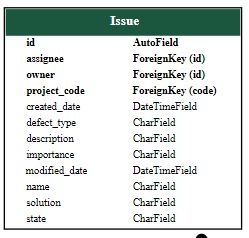
\includegraphics[scale=1.5]{issueModel}
	\caption{Issue modell diagrammja}
	\label{fig:issuemodel}
\end{figure}

Az \textbf{Issue} modellje már több mezőben is eltér a \textbf{Task} és \textbf{UserStory}-tól. A plusz mezők a korábbiakhoz képest, a \textit{defect\_type} és \textit{solution}. Előbbi a hiba típusát hívatott reprezentálni, utóbbi pedig egy rövid leírás a megoldásról. Ez is kapcsolódik egy projekthez és a létrehozójához, valamint ahhoz akihez hozzárendelik (opcionális).

\begin{itemize}
	\item \textit{id}: mezőazonosító (alapvetően generált)
	\item \textit{assignee}: idegen kulcs a hozzárendelt felhasználóra (lehet üres, \textbf{User} tábla)
	\item \textit{owner}: az issue-ot létrehozó felhasználó (idegen kulcs a \textbf{Profile} táblára)
	\item \textit{project\_code}: a projekt 6 karakter hosszú kódja (idegen kulcs, a \textbf{Project} tábla \textit{code} mezőjére mutat)
	\item \textit{created\_date}: a létrehozás dátuma
	\item \textit{defect\_type}: a hiba típusa (BUG, SYSTEM DEFECT - rendszer szintű, SPECIFICATION ISSUE - tervezési hiba, DEVELOPMENT ISSUE - fejelsztési hiba)
	\item \textit{modified\_date}: az utolsó módosítás dátuma
	\item \textit{name}: az epic neve (maximum 50 karakter hosszú)
	\item \textit{description}: egy leírás az issue-ról (maximum 250 karakter hosszú)
	\item \textit{importance}: fontosság (Low, Medium, High)
	\item \textit{soultion}: a megoldás rövid leírása (maximum 150 karakter)
	\item \textit{state}: aktuális állapot (OPEN, DONE, CLOSED)
\end{itemize}

Rendelkezik egy \textit{comment} mezővel is, amely több kommentet is össze kapcsol egy \textbf{Issue}-val (\textbf{ManyToMany} reláció, külön kapcsolati táblával). Ugyanilyen kapcsolatban áll a \textbf{Worklog} táblával is a \textit{work\_log} mezőn keresztül.

\subsection{Comment modell}

A \textbf{Projects} applikáción belül található a \textbf{Comments} modul is. Egy-egy \textbf{UserStory, Task, Issue} rendelkezhet kommentekkel különböző felhasználóktól. Ezekhez az egyes modellekben van idegen kulcsos mező, amely mutat egy-egy kommentre (\textbf{Many-To-Many} kapcsolat). 

\begin{figure}[H]
	\centering
	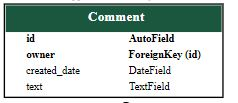
\includegraphics[scale=1.5]{commentModel}
	\caption{Comment modell diagrammja}
	\label{fig:commentModel}
\end{figure}

Mezői:

\begin{itemize}
	\item \textit{id}: mezőazonosító (alapvetően generált)
	\item \textit{owner}: a kommentelő felhasználó (idegen kulcs a \textbf{User} táblára)
	\item \textit{created\_date}: a létrehozás dátuma
	\item \textit{text}: a komment szövege (maximum 250 karakter hosszú)
\end{itemize}

\subsection{Worklog modell}

\begin{figure}[H]
	\centering
	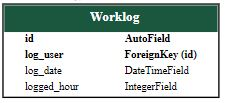
\includegraphics[scale=1.5]{worklogModel}
	\caption{Worklog modell diagrammja}
	\label{fig:worklogmodel}
\end{figure}

A munkaidő napló adatbázis reprezentációjául a \textbf{Worklog} modell szolgál. Munkaidő napló bejegyzést \textbf{UserStory-hoz, Task-hoz és Issue-hoz} tudunk létrehozni. Ezekhez az egyes modellek saját \textit{work\_log} mezőjével kapcsolódik. A mezői:

\begin{itemize}
	\item \textit{id}: mezőazonosító (alapvetően generált)
	\item \textit{log\_user}: a létrehozó felhasználója (idegen kulcs a \textbf{User} táblára)
	\item \textit{log\_date}: a létrehozás dátuma
	\item \textit{logged\_hour}: az órák száma ([0..8] intervallumba kell essen)
\end{itemize}

\section{Szerver réteg}

A szerver réteg jelen alkalmazásban a szolgáltatások (services) és nézetek (views) adják. Egy-egy applikáció a következő modulokból (gyakorlatilag fájlokból épül fel) :

\begin{itemize}
	\item \textit{admin.py}: A Django biztosít egy admin felületet az alkalmazás adatbázis szintű kezelésére. Egy adott modell akkor szerkezthető az admin oldalon, ha beregisztráljuk ebben a fájlban.
	\item \textit{apps.py}: Az egyes applikációk nevét tudjuk itt megadni, amivel tudunk rá hivatkozni a többi alkalmazásból (például: "projects.stories"), valamint egyéb alapkonfigurációkat az applikációról.
	\item \textit{migrations}: Ez egy almappa, amiben alap és későbbi (fájl nevében időponttal jelölt) adatbázis migrációk találhatók. Ezek a modellek változásaikor az adatbázis reprezentációjukon módosítanak annak megfelelően.
	\item \textit{templates}: A template-eket, azaz a HTML fájlokat tartalamzza, amik a böngészőben megjelenítendő Nézet rétehet adják. Lehetőség van a fő mappában (jelen esetben \textit{ScrumHelper}) létrehozni egyetlen tempaltes mappát és abban alkalamzásonként almappát, amelybe helyezzük a fájlokat,   de az újrafelhasználhatóság érdekében jobb megoldás minden ilyen fájlt és almappát az applikáció saját mappájában elhelyezni.
	\item \textit{constants.py}: nem kötelező fájl. Applikáció szintű konstansok tárolására használható.
	\item \textit{forms.py}: Szintén nem kötelező fájl. Ha használunk form-okat (például regisztrációra), akkor érdemes ebbe a fájlba elhelyezni ezeket.
	\item \textit{services.py}: A szolgáltatások helye. Ez sem kötelező, de ha az alkalamzáshoz például egy API-t (Application Programming Interface) akarunk fejelszteni, akkor helyesebb analógia a view-k helyett service-eket használni.
	\item \textit{tests.py}: Az egyes applikációk egységteszt modulja.
	\item \textit{views.py}: A view-k (nézetek) modulja. Ezek jelentik a közvetlen kapcsolatot az adatbázis/szolgáltatás réteg és a template-ek (a megjelenítés) között.
	\item \textit{urls.py}: Az applikációk szolgáltatásainak és view-inak az elérési útját tartalmazza (azaz a végpontokat, URL címeket).
\end{itemize}

A következő alfejezetekben az egyes applikációk szerver rétegébe tartozó részei lesznek részletezve (szolgáltatások, nézetek, végpontok, formulák).

\subsection{Login}

A \textbf{Login} applikáció a bejelentkeztetésért felelős. Alapvetően a keretrendszerben implementált bejelentkeztetést használja, illetve azt bővíti ki.

\begin{itemize}
	\item \textbf{Forms:}

	\begin{description}
		\item[SignUpForm:] A regisztrációs formula. \textbf{UserCreationForm}-ból van származtatva, amely a \textit{django.contrib.auth.forms} modulban van implementálva. A formulának hét mezője van: \textit{username, first\_name, last\_name, email, password1, password2, group}. Vannak megkötések az egyes mezőkre. A \textit{first\_name} csak 30 karakter hosszú lehet, nem kötelező megadni. Ugyanezek igazak a \textit{last\_name} mezőre is. Az \textit{email} mező egy maximum 254 karakter hosszú, email formátumú bemenetet fogad csak el. A \textit{password1} és \textit{password2} mezők jelszó mezők, amiknek egyezniük kell a formula véglegesítésekor. A \textit{group} egy olyan mezőtípus (\textbf{ChoiceField}, amely közvetlenül az adatbázisból kérdezi le a választási lehetőségeket (az \textit{auth\_groups} táblából).
		\item[ChangePassword:] A jelszóváltoztatáshoz használt formula. Ugyanazokkal a mezőkkel rendelkezik, mint a regisztrációs formula.
	\end{description}

	\item \textbf{Nézetek (views):}

	\begin{description}
		\item[CustomLoginView:] Erre azért van szükség, mert itt tudjuk megadni a \textit{redirect\_filed\_name} attribútummal, hogy hova navigáljon bejelenkezés után (jelen esetben: users/index.html).
		\item[index:] Az index oldal, azaz a "login/index.html" tartalmát jeleníti meg. 
\textbf{Végpontja:} "/" avagy "/login".
		\item[logout:] Meghívja a  \textit{django.contrib.auth.login} függvényt és visszanavigál a \textit{login} oldalra. 
\textbf{Végpontja:} "/logout/".
		\item[signup:] A regisztrációs formula segítségével biztosítja a felahsználó létrehozását. A "POST" HTTP üzenetet kap bemenetként, akkor ellenőrzi, hogy helyes-e a formula, majd lementi a felahsználót és hozzárendeli a megfelelő csoporthoz. Ezután visszajuttat az aktuálisan bejelentkezett felhasználó index oldalára. "GET" üzenet esetén csak egy üres forumlát biztosít kitöltésre a \textit{registration/signup.html} számára. 
\textbf{Végpontja:} "registration/signup/".
		\item[edit\_user:] Az egyes felhasználók szerkeztésére szolgál. Ugyanazt a formulát ahsznála, mint a regisztráció, csak itt "GET" üzenet esetén is a az ismert adatokkal kitöltve adja át a tempalte-nek. 
\textbf{Végpontja:} "edit\_user/<int:user\_id>/", azaz a bemenő paramétere egy felhasználói azonosító.
		\item[change\_pw:] A jelszóváltoztatást valósítja meg. Ehhez szintén egy user\_id-t vár bementként és a regisztrációs formulát használja. Azért van szükség mégis külön kezelni, mert nem midne felhasználónak van jogosultsága elérni a szerkeztést. 
\textbf{Végpontja:} "change\_pw/<int:user\_id>".
	\end{description}
\end{itemize}

\subsection{Projects}

A \textbf{Projects} applikáció a projektek megvalósítása. Ennek almappái a \textbf{Stories, Issues, Comments, Tasks, Epics} applikációk, de ezek külön fejezetkben leszek részletezve. A \textbf{Comments} applikáció lényegében csak a kommentek adatbázis reprezentációjára szolgál, saját szolgáltatásokkal és nézettel nem rendelkezik, így ez nem lesz részletezve ebben a fejezetben.

\begin{itemize}
	\item \textbf{Forms:}
	\begin{description}
		\item[CreateProjectForm:] A projekt létrehozásához használatos form. Mezői: \textit{name, code, release}, azaz a projekt neve, a projekt 6 karakter hosszú kódja és a release kódja.
		\item[CreateStoryForm:] A \textbf{Story} létrehozás form-ja. Mezői: \textit{name, project\_code, assignee, description, importance, epic}. A \textit{project\_code, assignee, epic} mezők \textbf{ModelChoiceField} típusúak, tehát egy megadott adathalmazból kínálnak fel opciókat. Az \textit{epic} és \textit{assignee} mezők kiválasztása nem kötelező.
		\item[CommentForm:] A kommentek létrehozásához használt form. Csak \textit{text} mezője van a komment szövegének lementéséhez.
		\item[CreateEpicForm:] Az \textbf{Epic} létrehozó formulája. Mezői: \textit{name, project\_code, description}, azaz a neve, a projekt kódja, amelyhez tartozik és egy leírás.
		\item[CreateWorklogform:] A \textbf{Worklog}, azaz munkanapló bejegyzés létrehozásához használt form. Mezők: \textit{log\_date, logged\_hour}. A feladattal végzett munkaidő és maga a munkanap.
		\item[CreateTaskForm:]  A \textbf{Task} létrehozás form-ja. Mezői: \textit{name, project\_code, assignee, description, importance, epic}. A \textit{project\_code, assignee, epic} mezők \textbf{ModelChoiceField} típusúak, tehát egy megadott adathalmazból kínál fel opciókat. Az \textit{epic} és \textit{assignee} mezők kiválasztása nem kötelező.
		\item[CreateIssueForm:] Az \textbf{Issue} létrehozás form-ja. Mezői: \textit{name, project\_code, assignee, description, importance, epic, defect\_type,solution}. A \textit{project\_code, assignee, epic} mezők \textbf{ModelChoiceField} típusúak, tehát egy megadott adathalmazból kínál fel opciókat. Az \textit{epic} és \textit{assignee} mezők kiválasztása nem kötelező. A \textit{defect\_type} mező is egy \textbf{ChoiceField}, tehát adott lehetőségekből lehet választani: BUG, SYSTEM DEFECT, DEVELOPMENT, SPECIFICATION ISSUE. Utóbbi értékek egy konstansban találhatóak a \textit{contants.py} modulban, az \textit{ISSUE\_CHOICES} változóban.
	\end{description}
	\item \textbf{Szolgáltatások (services):}
	\begin{description}
		\item[get\_issues\_for\_project:] Bemeneti paramétere: \textit{project\_id}. A megkapott projekt azonosítóhoz lekérdezi magát a projektet, a hozzátartozó story-kat, task-okat, issue-kat, epic-eket és feltöltött dokumentumokat. Ezeket egy \textit{context} nevű, dictionary típusú változóba gyűjti, ami a visszatérési értéke a függvénynek.
		\item[delete\_project:] Bemeneti paraméter: \textit{project\_id}. A megkapott projekt azonosító alapján megkeresi az adatbázisban a projektet és kitörli.
	\end{description}
	\item \textbf{Nézetek (views):}
	\begin{description}
		\item[index:] Lekérdezi az adatbázisban található összes projektet. A \textit{django.core.paginator} modul beli \textbf{Paginator} segítségével oldalakra osztja az eredményeket (jelen beállítás szerint ötösével). Ennek megoldása a \ref{src:paginator}. kódrészletben látható. Az így rendezett projekt listát hozzárendeli a "projects/index.html"-hez. \textbf{Végpont:} "projects/".
		\item[detail:] Bemenő paraméter: \textit{request, project\_id}. Utóbbival meghívja a \textit{get\_issues\_for\_project} szolgáltatást és az ebből megszerzett \textit{context} változót hozzárendeli a "projects/details.html" oldalhoz. \textbf{Végpont}: "projects/<int:project\_id>/".
		\item[project\_new:] Új projekt létrehozását kezelő view. "GET" üzenet esetén biztosítja az üres \textbf{CreateProjectForm}-ot, "POST" üzenet esetén ellenőrzi és lementi az adatokat. \textbf{Végpont:} "projects/new/".
		\item[project\_edit:] A bemeneti paraméterként megkapott \textit{project\_id} alapján megkeresi az adatbázisban a projektet, majd egy \textbf{CreateProjectForm}-ot ad vissza az ismert adatokkal kitöltve "GET" üzenet esetén. "POST" üzenet esetén frissíti az adatbázisban a projekt adatait. \textbf{Végpont:} "projects/<int:project\_id>/edit".
		\item[delete:] A paraméterül kapott \textit{project\_id}-val meghívja a \textit{delete\_project} szolgáltatást. \textbf{Végpont:} "projects/delete/<int:project\_id>/".
		\item[upload\_doc:] Bemeneti paramétere: \textit{project\_id}. Az adott projekthez való dokumentum feltöltést végzi. A fájlt a \textit{request} paraméter FILE attribútumában kapja meg. \textbf{Végpont:} "projects/<int:project\_id>/upload\_doc".
		\item[delete\_doc:] Bementben megkapja a \textit{project\_id}-ját és a \textit{doc\_id}-ját. E kettő segítségével törli az adatbázisból a fájlt. \textbf{Végpont:} "projects/<int:project\_id>/delete\_doc/<int:doc\_id>".
		\item[kanban\_board]: Legyűjti a az összes story-t, task-ot, issue-ot a kanban táblához (amelyek az elmúlt 30 napban módosultak). \textbf{Végpont:} "projects/kanban/".
		\item[get\_chart\_data:] Összeszedi az adatbázisból a szükséges adatokat a kanban körgrafikonos kimutatásához. \textbf{Végpont:} "projects/kanban\_chart".
	\end{description}
\end{itemize}

\pagebreak

\lstset{caption={Az adatbázisban található projektek listájának oldalakra tördelése a Paginator segítségével}, label=src:paginator}
\begin{lstlisting}[language={python}]

def index(request):
    projects_list = Project.objects.all().order_by('-created_date')
    paginator = Paginator(projects_list, 5)

    page_number = request.GET.get('page',1)
    projects = paginator.get_page(page_number)

    context = {
        'project_list': projects_list,
        'projects': projects,
    }
    return render(request, 'projects/index.html', context)

\end{lstlisting}

\subsection{Epics}

Az \textbf{Epics} applikáció az epic-ek megvalósítása. 

\begin{itemize}
	\item \textbf{Szolgáltatások (services):}
	\begin{description}
		\item[]
	\end{description}
	\item \textbf{Nézetek (views):}
	\begin{description}
		\item[index:]
	\end{description}
\end{itemize}